
\documentclass{article} % For LaTeX2e
\usepackage{style,times}
\usepackage{amsmath,amsfonts,bm,amssymb}
\usepackage{algorithm}
\usepackage{algpseudocode}

%%%%% customized by shuo begin
\usepackage{amsthm}
\DeclareMathOperator*{\argmax}{argmax}
\usepackage{hyperref}
\usepackage{url}
\usepackage{tikz}
\usepackage{subcaption}

\newcommand{\bellman}{\mathcal{T}^\pi}
\newcommand{\bellmanopt}{\mathcal{T}^*}
\newtheorem{theorem}{Theorem}
\newtheorem{definition}{Definition}
\newtheorem{proposition}{Proposition}
\newtheorem{corollary}{Corollary}

\newcommand{\red}[1]{\textcolor{red}{#1}}
%%%% customized by shuo end

\title{Understanding Bellman Equations}

\author{Shuo Liu \\
Computer Science\\
Northeastern University\\
\texttt{shuo.liu2@northeastern.edu} \\
}

\iclrfinalcopy % Uncomment for camera-ready version, but NOT for submission.
\begin{document}

\maketitle
\begin{abstract}
This article covers Bellman Equation, its RL specializations, and generalizations.
\end{abstract}

%\tableofcontents \clearpage % this should be removed in the camera-ready version

\section{Bellman Equation and Operator}

\subsection{Definition}

The Bellman Equation and optimal Bellman Equation for V-values are, \cite{sutton2018reinforcement},\footnote{The Bellman Equations shown in the main article are stochastic, the deterministic one can be derived as, $V(s) = \max_{a} \left\{ R(s, a) + \gamma V(s')\right\}$, where $s'\gets T(s,a)$ is a deterministic succeeding state of $s$ following $a$.}
\begin{equation}
	\begin{aligned}
	V^\pi(s) &\doteq \mathbb{E}_{a \sim \pi(\cdot|s)} \left[ Q^\pi(s, a) \right], \\
    &= \mathbb{E}_{a \sim \pi(\cdot|s)} \left[ R(s, a) + \gamma \mathbb{E}_{s' \sim P(\cdot|s,a)} \left[V^\pi(s')\right] \right],  \\
	V^*(s) &\doteq \max_{a} \left[ Q^*(s, a) \right], \\
    &= \max_{a} \left[ R(s, a) + \gamma \mathbb{E}_{s' \sim P(\cdot|s,a)} \left[V^*(s')\right] \right].
\end{aligned}
\end{equation}
and the Bellman Equation and optimal Bellman Equation for Q-values are,
\begin{equation}
	\begin{aligned}
    Q^\pi(s, a) &\doteq R(s, a) + \gamma \mathbb{E}_{s'\sim P(\cdot|s,a)} \left[V^\pi(s')\right], \\
    &= R(s, a) + \gamma \mathbb{E}_{s'\sim P(\cdot|s,a)} \left[\mathbb{E}_{a'\sim\pi(a'|s')} Q^\pi(s', a')\right]. \\
    Q^*(s, a) &\doteq R(s, a) + \gamma \mathbb{E}_{s'\sim P(\cdot|s,a)} \left[V^*(s')\right], \\
    &= R(s, a) + \gamma \mathbb{E}_{s'\sim P(\cdot|s,a)} \left[\max_{a'} Q^*(s', a')\right]. 
\end{aligned}
\end{equation}
where $V^\pi(s)$ and $Q^\pi(s,a)$ are value representations following policy $\pi$, e.g., vectors and functions.
\begin{equation}
	\tilde{\pi}(s) \doteq \argmax_a Q^\pi (s,a).
\end{equation}
Bellman Equations establish relations between states and succeeding states, which can be applied as updating rules for value prediction. A succinct representation is to define the Bellman Equation as a unary mathematical operator. The V-value Bellman and optimal Bellman Operators are,
\begin{equation}
	\begin{aligned}
    (\bellman \circ V^\pi)(s) &\doteq \mathbb{E}_{a \sim \pi(\cdot|s)} \left[ R(s, a) + \gamma \mathbb{E}_{s' \sim P(\cdot|s,a)} \left[V^\pi(s')\right] \right], \\
    (\bellmanopt \circ V^\pi)(s) &\doteq \max_a \left[ R(s, a) + \gamma \mathbb{E}_{s' \sim P(\cdot|s,a)} \left[V^\pi(s')\right] \right]. 
\end{aligned}
\end{equation}
The Bellman and optimal Bellman Operators $\bellman$ for Q-values are,
\begin{equation}
	\begin{aligned}
    (\bellman \circ Q^\pi)(s, a) &\doteq R(s, a) + \gamma \mathbb{E}_{s' \sim P(\cdot|s,a)} \left[ \mathbb{E}_{a' \sim \pi(a'|s')} Q^\pi(s', a') \right],  \\
    (\bellmanopt \circ Q^\pi)(s, a) &\doteq R(s, a) + \gamma \mathbb{E}_{s' \sim P(\cdot|s,a)} \left[ \max_{a'} Q^\pi(s', a') \right].
\end{aligned} 
\end{equation}

\paragraph{Curse of Dimension}

Why do we mostly use MDP (where the future evolution is independent of its history) and hence Bellman Equations to model RL problems? \cite{bellman1957dynamic} coined the ``curse of dimension'', which describes the exponential increase in the state space size as dimensionality grows, making calculations extremely complex. Breaking this curse often requires altering the problem or its constraints, though complete solutions are not always achievable.

\textit{For convenience, we use Q-value as the representative in the following parts of this article.}

\subsection{Important Properties}

\begin{proposition} [$\gamma$-contraction]
	Given any $Q,\ Q' \mapsto \mathbb{R}^{|\mathcal{S}| \times |\mathcal{A}|}$, Bellman Operators are $\gamma$-contraction Operators in $L^\infty$ norm,
	\begin{equation}
	\begin{aligned}
		\|\mathcal{T}^\pi \circ Q - \mathcal{T}^\pi \circ Q'\|_\infty &\leqslant \gamma \|Q-Q'\|_\infty,\\
		\text{and }\|\mathcal{T}^* \circ Q - \mathcal{T}^* \circ Q'\|_\infty &\leqslant \gamma \|Q-Q'\|_\infty.
	\end{aligned}
	\end{equation}
\end{proposition}

\begin{corollary} [Fixed-point Iteration] \label{them:fixpoint}
	For any $Q^0 \mapsto \mathbb{R}^{|\mathcal{S}| \times |\mathcal{A}|}$, after $k\to \infty$ iterations of Bellman transformation, $Q^{\pi, \infty} \doteq \lim_{k \to\infty} (\mathcal{T}^\pi)^k \circ Q^0$, or $ Q^{*, \infty} \doteq \lim_{k\to\infty} (\mathcal{T}^*)^k \circ Q^0$, according to Banach's Fixed Point Theorem,
	\begin{equation}
	\begin{gathered}
		Q^{\pi, \infty}=Q^{*, \infty}=Q^*, \\ \text{which \textbf{uniquely} satisfies } \mathcal{T}^\pi \circ Q^*  = Q^*, \text{ or } \mathcal{T}^* \circ Q^*  = Q^*.
	\end{gathered}
	\end{equation}
\end{corollary}

\begin{theorem} [Fundamental theorem] \label{them:fundamental}
	Any memoryless policy that is greedy to $Q^*$ (\textbf{deterministically} maximizes) is optimal \cite{szepesvari2010algorithms},
	\begin{equation}
	\begin{aligned}
		\tilde{\pi}^{*} \doteq \argmax_aQ^* = \pi^*.
	\end{aligned}
	\end{equation}
\end{theorem}

\begin{proposition} [Monotone]
	Bellman Operators are monotonic. For any Q-values $Q,Q' \mapsto \mathbb{R}^{|\mathcal{S}| \times |\mathcal{A}|}$,
	\begin{equation}
	\begin{aligned}
		\left (Q\leqslant Q'\right ) &\Leftrightarrow \left (\mathcal{T}^\pi \circ Q\leqslant \mathcal{T}^\pi \circ Q'\right ),\\
		\left (Q\leqslant Q'\right )&\Leftrightarrow \left (\mathcal{T}^* \circ Q\leqslant \mathcal{T}^* \circ Q'\right ).
	\end{aligned}
	\end{equation}
\end{proposition}

\section{Bellman Backup for Planning}

\subsection{Dynamic Programming}

According to the Fundamental Theorem, we can find $\pi^*$ efficiently once having access to $Q^*$, without the need to find the policy whose Q-function \textbf{dominates} the others' brute-force-ly. To avoid the Bellman Curse of Dimensionality, we can apply Dynamic Programming (DP) methods to solve MDPs by keeping track of Q-values during calculations, thanks to Bellman recursions.

\paragraph{Value Iteration} Value iteration (so-called backward induction) involves iteratively applying $\mathcal{T}^*$ to arbitrarily initialized values $Q^0$ until convergence. According to Corollary~\ref{them:fixpoint} and Theorem~\ref{them:fundamental}, value iteration converges to $Q^*$ as $k \to \infty$, then an optimal policy $\pi^*$ can be derived by greedifying $Q^*$.

\paragraph{Policy Iteration} Policy iteration starts with an arbitrary policy $\pi^0$ and values $Q^0$. In each iterative step $k$, $Q^{\pi, k}$ is calculated by applying Bellman Operator $\mathcal{T}^{\pi, k}$ that follows current policy ${\pi^k}$ to $Q^{\pi, {k-1}}$ from the last iteration, and then $\pi^{k+1}$ is derived from greedifying $Q^{\pi, k}$. This process is repeated until convergence, and policy iteration can produce optimal policy after sufficient iterations.
 

\section{Bellman Residual for Learning}

\subsection{TD-Learning with Look-up Table}

When the transition model is unavailable (model-free), we can use the residuals (RHS minus LHS) of the Bellman Equations as learning objective,
\begin{equation}
\begin{aligned}
	(\mathcal{B}^\pi\circ Q) (s,a) &\doteq  r + \gamma Q(s', \pi(s')) - Q(s, a),\\
	(\mathcal{B}^*\circ Q) (s,a) &\doteq  r + \gamma \max_{a'} Q(s', a') - Q(s, a).
\end{aligned}
\end{equation}
Assuming that our sampling and parameter updating roughly follow the true state distribution $\mu(s)$, the expectation of Bellman residual will be closed to zero at the optima. This approach is often called temporal difference (TD) learning. 

\paragraph{TD-learning} In TD-learning with learning rate $\alpha$, the update rule for Q-values is,
\begin{equation}
Q(s, a) \leftarrow Q(s, a) + \alpha (\mathcal{B}^\pi\circ Q) (s,a). \label{eq:td-learning}
\end{equation}
According to Stochastic Approximation Theorem, let $k$ be the visitation times of state-action pair, and learning rates $0 \leqslant \alpha^k < 1$ satisfies $\forall (s, a)$, $\sum_{k=1}^\infty \alpha^k(s, a) = \infty,\sum_{k=1}^\infty [\alpha^k(s, a)]^2 < \infty$. Following TD-learning updates, $Q^{\pi, k}(s, a)$ converges to $Q^*(s, a)$ as $k \to \infty$ (\cite{jaakkola1994convergence}).

\paragraph{Q-learning} In Q-learning that relies on optimal Bellman Equation, the Q-value update is,
\begin{equation}
Q(s, a) \leftarrow Q(s, a) + \alpha (\mathcal{B}^*\circ Q) (s,a). \label{eq:q-learning}
\end{equation}
According to Stochastic Approximation Theorem, let $k$ be the visitation times of state-action pair, and learning rates $0 \leqslant \alpha^k < 1$ satisfies $\forall (s, a)$, $\sum_{k=1}^\infty \alpha^k(s, a) = \infty, \sum_{k=1}^\infty [\alpha^k(s, a)]^2 < \infty$. Following Q-learning updates, $Q^{*, k}(s, a)$ converges to $Q^*(s, a)$ as $k \to \infty$ (\cite{watkins1992qlearning}). The deep version of Q-learning algorithm, Deep Q-Network (DQN), is shown in Appendix.

However, the nice property of convergence only holds in the tabular case and cannot be extended to a function approximation as discussed later.

\subsection{TD-learning with Function Approximation}

To introduce generalization to the value function, we represent the approximated Q-value in a parameterized functional form. Our goal is to minimize the mean squared value error,
\begin{equation}
    \mathcal{L}(\theta) = \frac{1}{2}\sum_{s \in \mathcal{S}} \mu(s) \Big[ Q^\text{target} - Q_\theta(s, a) \Big]^2,
\end{equation}
where $Q^\text{target}$ is the ground truth and $Q_\theta$ is the prediction. Just like TD-learning, the Bellman residual can be applied for the value function approximation.

\paragraph{Semi gradient for Bellman Residual}

Similar to stochastic gradient methods with unbiased target estimators, if we use the Bellman Equation to get target Q-value $Q^\text{target}$, but here we just ignore its potential gradient change, the gradient ascent for Bellman residual is,
\begin{equation}
\begin{aligned}
    \Delta_\text{semi} \theta &= -\frac{1}{2}\alpha \nabla_\theta  \Big[Q^\text{target} - Q_\theta(s, a) \Big]^2 \\ 
    &= \alpha \Big[Q^\text{target} - Q_\theta(s, a) \Big] \nabla_\theta Q_\theta(s, a), \text{ where } Q^\text{target} = r + \gamma Q_{\red{\theta}}(s', a')\label{eq:semi-grad}
\end{aligned}
\end{equation}
Since we neglects a part of the gradient of $Q^\text{target}$, it is called semi gradient for Bellman residual ($\theta$ in red). Though semi-gradient methods are fast and simple, they could have divergence issue, e.g., Baird's counter-example (the star problem).

\paragraph{Full Gradient for Bellman Residual}

The full Bellman residual gradient should include all gradient components, including the gradient of the target estimation, 
\begin{equation}
\begin{aligned}
    \Delta_\text{full} \theta &= -\frac{1}{2}\alpha \nabla_\theta  \Big[ r + \gamma Q_\theta(s', a') - Q_\theta(s, a) \Big]^2 \\
    & = -\alpha \Big[ r + \gamma Q_\theta(s', a') - Q_\theta(s, a) \Big] \Big[ \gamma\nabla_\theta Q_\theta(s', a') - \nabla_\theta Q_\theta(s, a) \Big].
\end{aligned}
\end{equation}
If the approximation system is general enough and the value functions are continuous, the full Bellman residual gradient is guaranteed to converge to the optima. However, this is at the sacrifice of learning speed, as illustrated by the hall problem.

\paragraph{Hybrid Gradient for Bellman Residual} In contrast to Figure~\ref{subfig:sg-increase} where $\Delta_\text{semi}$ boosts $\Delta_\text{full}$, Figure~\ref{subfig:sg-decrease} represents the case where the semi gradient may diverge. \cite{baird1995residual} combined these 2 methods: to keep stable, $\Delta_\text{B}$ should stay in the same direction as $\Delta_\text{full}$ (above the perpendicular axis); meanwhile, $\Delta_\text{B}$ should stay as close as possible to $\Delta_\text{semi}$ to increase learning speed.
\begin{equation}
\begin{aligned}
	\Delta_\text{B} \theta &= (1 - \omega)  \cdot \Delta_\text{semi}\theta + \omega \cdot \Delta_\text{full}\theta, \\
	&=-\alpha \Big[ r + \gamma Q_\theta(s', a') - Q_\theta(s, a) \Big] \Big[\omega \gamma \nabla_\theta Q_\theta(s', a') - \nabla_\theta Q_\theta(s, a) \Big],\\
	&\text{s.t.,} \ \Delta_\text{B}\theta \cdot \Delta_\text{full}\theta\geqslant 0 \Leftrightarrow \omega \geqslant \frac{\Delta_\text{semi}\theta \cdot \Delta_\text{full}\theta}{\Delta_\text{semi}\theta \cdot \Delta_\text{full}\theta - \Delta_\text{full}\theta \cdot \Delta_\text{full}\theta}.
\end{aligned} 
\end{equation}

\begin{figure}[h!]
\centering
\begin{subfigure}{0.45\textwidth}
\centering
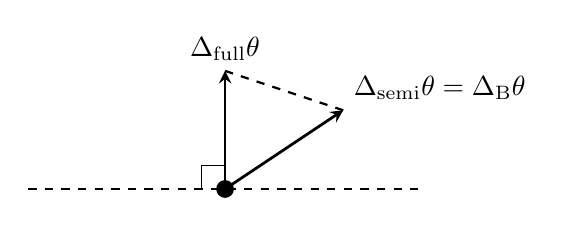
\begin{tikzpicture}
    \draw[dashed] (-2.5,0) -- (2.5,0);
    \draw[-] (-0.3,0.3) -- (-0.3,0);
    \draw[-] (-0.3,0.3) -- (0,0.3);
    \draw[->, thick, >=stealth, line width=1pt] (0,0) -- (0,1.5) node[above] {$\Delta_\text{full}\theta$};
    \draw[->, thick, >=stealth, line width=1pt] (0,0) -- (1.5,1) node[above right] {$\Delta_\text{semi}\theta=\Delta_\text{B}\theta$} node[above right] {};
    \draw[dashed, thick] (1.5,1) -- (0,1.5);
    \filldraw (0,0) circle (3pt);
\end{tikzpicture}
\caption{Gradient ascent by semi-gradient.} \label{subfig:sg-increase}
\end{subfigure}
\hfill
\begin{subfigure}{0.45\textwidth}
\centering
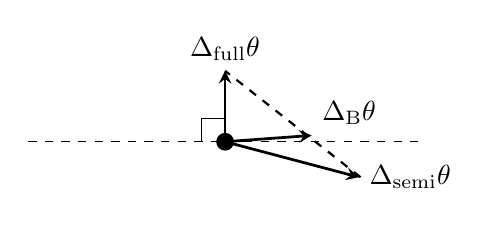
\begin{tikzpicture}
    \draw[dashed] (-2.5,0) -- (2.5,0);
    \draw[-] (-0.3,0.3) -- (-0.3,0);
    \draw[-] (-0.3,0.3) -- (0,0.3);
    \draw[->, thick, >=stealth, line width=1pt] (0,0) -- (0,.9) node[above] {$\Delta_\text{full}\theta$};
    \draw[->, thick, >=stealth, line width=1pt] (0,0) -- (1.7,-.45) node[right] {$\Delta_\text{semi}\theta$};
    \draw[->, thick, >=stealth, line width=1pt] (0,0) -- (1.1,0.08) node[above right] {$\Delta_\text{B}\theta$};
    \draw[dashed, thick] (1.72,-.45) -- (0,.9);
    \filldraw (0,0) circle (3pt);
\end{tikzpicture}
\caption{Gradient descent by semi-gradient.} \label{subfig:sg-decrease}
\end{subfigure}
\caption{Epoch-wise gradient vectors for Bellman residual gradients.}
\end{figure}

\section{Bellman Generalizations}

\subsection{Soft Bellman Equation}
The Soft Bellman Equation incorporates an entropy regularization term, encouraging exploration by penalizing overly deterministic policies. It is useful where balancing exploration and exploitation is critical, such as environments with sparse rewards or high uncertainty.
\begin{equation}
Q(s, a) = R(s,a) + \gamma \mathbb{E}_{a'\sim \pi(\cdot|s'), s' \sim P(\cdot | s, a)} \Big[Q(s', a') - \lambda \log\pi(\cdot|s') \Big],
\end{equation}
where $\lambda$ controls the weight of the entropy term $\mathcal{H}(\cdot|s)$.

\subsection{Continuous-Time Bellman Equation}
Hamilton-Jacobi-Bellman (HJB) Equation is the continuous-time analogue of the Bellman Equation and used in problems involving continuous state and action spaces. Given system dynamics $f(s, a)$, 
\begin{equation}
\frac{\partial Q(s,a)}{\partial t} + \max_a \Big[ R(s,a) + \nabla_s Q(s,a)^T f(s, a) \Big]=0.
\end{equation}

\subsection{Distributional Bellman Equation}
The Distributional Bellman Equation models the return as a distribution $\mathcal{Q}$, which is particularly useful in risk-sensitive scenarios with specific demands of quantifying the variability of returns,
\begin{equation}
\mathcal{Q}(s, a) \stackrel{\text{D}}{=} R(s,a) + \gamma \mathcal{Q}(s', a'),
\end{equation}
where $\mathcal{Q}$ is distributional expected returns, and $\stackrel{\text{D}}{=}$ denotes equility in distribution.

\subsection{Multi-Agent Bellman Equation}
The Multi-Agent (MA) Bellman Equation generalizes the Bellman Equation to cooperative MA systems, where multiple agents collaborate to achieve a common goal.

\paragraph{Joint Bellman Equation} The Joint MA Bellman Equation models the group of agents as an entity, considering their collective actions $\mathbf{a} = (a_1, \dots, a_N)$ and expected returns $Q$,
\begin{equation}
Q(s, \mathbf{a}) = R(s, \mathbf{a}) + \gamma \mathbb{E}_{\mathbf{a}' \sim \pi(\cdot |s'), s' \sim P(\cdot | s, \mathbf{a})} \Big[ Q(s', \mathbf{a'}) \Big].
\end{equation}

\paragraph{Individual Bellman Equation} The Individual Bellman Equation computes $Q_i$ for each agent, assuming that agents' execution and rewards are independent (but observing a shared reward $R(s, \mathbf{a})$),
\begin{equation}
Q_i(s, a_i) = R(s, \mathbf{a}) + \gamma \mathbb{E}_{a_i' \sim \pi_i(\cdot |s'), s' \sim P(\cdot | s, a_i)} \Big[ Q_i(s', a_i') \Big].
\end{equation}

\subsection{Multi-Task Bellman Equation}
The Generalized Bellman Equation extends the Bellman Equation to include additional objectives. It is particularly useful in multi-task learning, constrained RL or hierarchical RL with additional objectives $\phi(s, a)$ or constraints $\phi(s, a)\gets\lambda c(s, a)$ alongside the primary goal,
\begin{equation}
Q(s, a) = R(s,a) + \phi(s, a) + \gamma \mathbb{E}_{a' \sim \pi(\cdot |s'), s' \sim P(\cdot | s, a)} \Big[ Q(s', a') \Big].
\end{equation}

\clearpage

\bibliography{ref}
\bibliographystyle{ref}

\newpage
\appendix

\section{Deep Q-Network}

Deep Q-Network (DQN) approximates the Q-function with a target network to stabilize training.

\begin{algorithm}[H]
    \centering 
    \caption{Deep Q-learning with Experience Replay}\label{alg:dqn}
    \begin{algorithmic}[1]
    \State \textbf{Initialize}: parameter $\theta$ for Q-network $Q_{\theta}$, target Q-network $\theta'\leftarrow \theta$, replay memory $\mathcal{D}$
    \For{each episode}
        \State Choose $s_0$ from $\mathcal{S}$ as initial state
        \For{$t=0$ to $T-1$}
        \State Take action $a_t$ according to policy derived by $Q$ (e.g. $\epsilon$-greedy)
        \State Observe reward $r_{t+1}$ and next state $s_{t+1}$
        \State Store transition $(s_t, a_t, r_{t+1}, s_{t+1})$ into $\mathcal{D}$
        \For{each mini-batch of $N$ transitions $\{s_i, a_i, r_{i+1}, s_{i+1}\}$}
        \State $\delta_i\leftarrow \underbrace{r_{i+1} +\gamma \max_{a'} Q_{\theta'}(s_{i+1}, a')}_{\text{target Q prediction}} - Q_{\theta}(s_i, a_i)$
        \State $\theta \leftarrow \theta + \frac{1}{N} \sum_i \alpha \delta_i \nabla_{\theta} Q_{\theta}(s_i, a_i)$
        \EndFor
        \State $\theta'\leftarrow \tau \theta' + (1-\tau) \theta$
        \EndFor
    \EndFor
\State \Return value function $Q$
\end{algorithmic}
\end{algorithm}

%\section{Theorems}
%
%\subsection{Banach Fixed-Point Theorem}
%
%\begin{theorem} \label{them:banach}
%Let $(X, d)$ be a non-empty complete metric space with a contraction mapping $T : X \rightarrow X$. Then $T$ admits a unique \textit{fixed-point} $x^* \in X$ (i.e. $T(x^*) = x^*$). Furthermore, $x^*$ can be found as follows: start with an arbitrary element $x_0 \in X$ and define a sequence $(x_n)_{n \in \mathbb{N}}$ by $x_n = T(x_{n-1})$ for $n \geq 1$. Then $\lim_{n \to \infty} x_n = x^*$.
%\end{theorem}
%
%The proof can find in \cite{szepesvari2010algorithms}
%
%\subsection{Stochastic Approximation Theorem}
%
%\section{Examples}
%
%\subsection{Baird's Counterexample}
%
%The star problem.


\end{document}
